\chapter{Présentation de l'entreprise d'accueil}
\section{Orange Business}
	Orange Business (anciennement Orange Business Services) est une filiale et une marque commerciale du groupe Orange qui fournit, en France et dans le monde, des services de communication intégrée aux entreprises dans les domaines du cloud computing, des télécommunications, des communications unifiées et de la collaboration.\\
	Orange Business regroupe les activités business to business des différentes filiales françaises et internationales du groupe Orange.\cite{orange_business}\\
	
	Orange Business est une identité commerciale du groupe Orange qui a été constituée le 1er juin 2006 (sous le nom d'Orange Business Services)2, afin d'offrir une marque unique des services de télécommunication (données, téléphonie et convergence) et informatiques pour les entreprises. Elle opère dans 220 pays et territoires et emploie plus de 21 000 personnes réparties sur 166 pays3.\\
	
	Orange Business est le résultat de la consolidation et du regroupement sous une seule marque, d’entités issues de trois entreprises aujourd’hui dissoutes : France Telecom, Equant et Wanadoo2.\\
	
	Le 16 février 2023, Christel Heydemann, la directrice générale du groupe Orange, annonce qu'Orange Business Services se nommera désormais tout simplement Orange Business.\cite{orange_business}\\
	
	Les lignes qui suivront, seront consacrées à Orange Business Nantes.
	
\section{L'équipe WAT} % Developpement web %
	En fonction des technologies utilisées, Orange Business Nantes est répartie en plusieurs équipes (WAT, BIM, PIX, TED et TM).\\
	
	L'équipe WAT(Web Applications Team), celle dans laquelle je fais partie, est spécialisée dans le pilotage et le développement d'applications Web basées sur les technologies PHP, dont le framework Symfony, ou des CMS, dont drupal et Wordpress.\\
	
	L'équipe est composée de :
	\begin{itemize}
		\item \textbf{Chefs de projets} : responsables du bon déroulement des projets.\\
		\item \textbf{Experts techniques} : ils ont un rôle transverse dans l'équipe en intervenant sur plusieurs projets. Leurs activités principales : support technique aux projets, avant-vente, mise en place des environnements techniques, de la CI/CD, veille techno, ...\\
		\item 	\textbf{Développeurs} : codent les fonctionnalités souhaitées sur les projets.\\
	\end{itemize}
	\begin{center}
		
\includegraphics[scale=0.4]{chap_1/WAT-logo.png}
		\captionof{figure}{Equipe WAT}
		\label{Equipe WAT}
	\end{center}
\section{Organigramme}
		L'illustration ci-dessous permet de résumer en une image les paragraphes ci-dessus décrivant l'entreprise.\\
		\begin{center}
			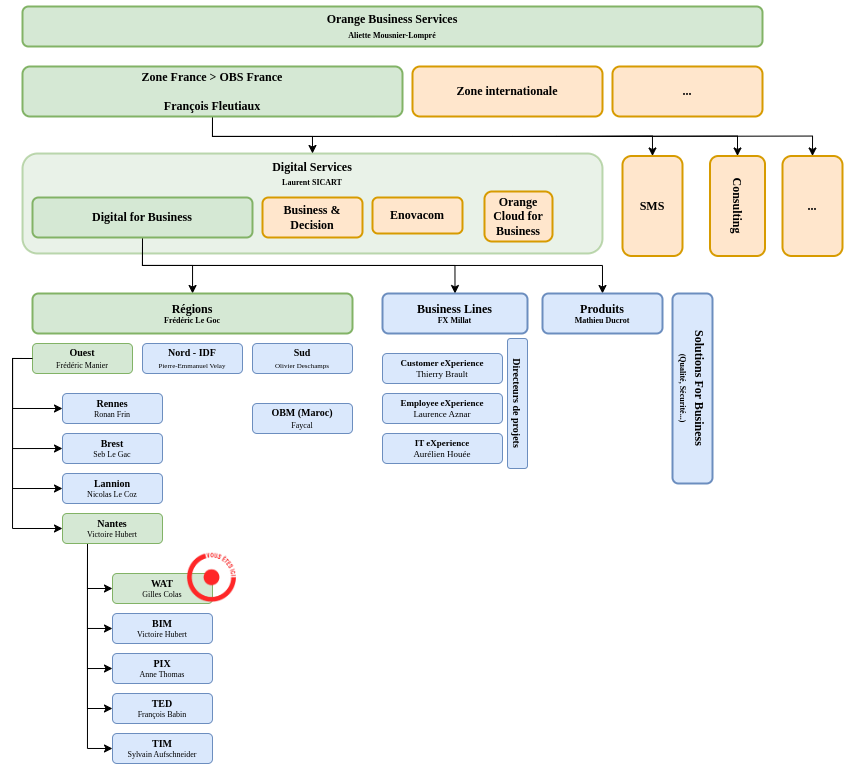
\includegraphics[scale=0.6]{chap_1/organigramme.png}
			\captionof{figure}{Organigramme}
			\label{Organigramme}
		\end{center}